\documentclass[1p]{elsarticle_modified}
%\bibliographystyle{elsarticle-num}

%\usepackage[colorlinks]{hyperref}
%\usepackage{abbrmath_seonhwa} %\Abb, \Ascr, \Acal ,\Abf, \Afrak
\usepackage{amsfonts}
\usepackage{amssymb}
\usepackage{amsmath}
\usepackage{amsthm}
\usepackage{scalefnt}
\usepackage{amsbsy}
\usepackage{kotex}
\usepackage{caption}
\usepackage{subfig}
\usepackage{color}
\usepackage{graphicx}
\usepackage{xcolor} %% white, black, red, green, blue, cyan, magenta, yellow
\usepackage{float}
\usepackage{setspace}
\usepackage{hyperref}

\usepackage{tikz}
\usetikzlibrary{arrows}

\usepackage{multirow}
\usepackage{array} % fixed length table
\usepackage{hhline}

%%%%%%%%%%%%%%%%%%%%%
\makeatletter
\renewcommand*\env@matrix[1][\arraystretch]{%
	\edef\arraystretch{#1}%
	\hskip -\arraycolsep
	\let\@ifnextchar\new@ifnextchar
	\array{*\c@MaxMatrixCols c}}
\makeatother %https://tex.stackexchange.com/questions/14071/how-can-i-increase-the-line-spacing-in-a-matrix
%%%%%%%%%%%%%%%

\usepackage[normalem]{ulem}

\newcommand{\msout}[1]{\ifmmode\text{\sout{\ensuremath{#1}}}\else\sout{#1}\fi}
%SOURCE: \msout is \stkout macro in https://tex.stackexchange.com/questions/20609/strikeout-in-math-mode

\newcommand{\cancel}[1]{
	\ifmmode
	{\color{red}\msout{#1}}
	\else
	{\color{red}\sout{#1}}
	\fi
}

\newcommand{\add}[1]{
	{\color{blue}\uwave{#1}}
}

\newcommand{\replace}[2]{
	\ifmmode
	{\color{red}\msout{#1}}{\color{blue}\uwave{#2}}
	\else
	{\color{red}\sout{#1}}{\color{blue}\uwave{#2}}
	\fi
}

\newcommand{\Sol}{\mathcal{S}} %segment
\newcommand{\D}{D} %diagram
\newcommand{\A}{\mathcal{A}} %arc


%%%%%%%%%%%%%%%%%%%%%%%%%%%%%5 test

\def\sl{\operatorname{\textup{SL}}(2,\Cbb)}
\def\psl{\operatorname{\textup{PSL}}(2,\Cbb)}
\def\quan{\mkern 1mu \triangleright \mkern 1mu}

\theoremstyle{definition}
\newtheorem{thm}{Theorem}[section]
\newtheorem{prop}[thm]{Proposition}
\newtheorem{lem}[thm]{Lemma}
\newtheorem{ques}[thm]{Question}
\newtheorem{cor}[thm]{Corollary}
\newtheorem{defn}[thm]{Definition}
\newtheorem{exam}[thm]{Example}
\newtheorem{rmk}[thm]{Remark}
\newtheorem{alg}[thm]{Algorithm}

\newcommand{\I}{\sqrt{-1}}
\begin{document}

%\begin{frontmatter}
%
%\title{Boundary parabolic representations of knots up to 8 crossings}
%
%%% Group authors per affiliation:
%\author{Yunhi Cho} 
%\address{Department of Mathematics, University of Seoul, Seoul, Korea}
%\ead{yhcho@uos.ac.kr}
%
%
%\author{Seonhwa Kim} %\fnref{s_kim}}
%\address{Center for Geometry and Physics, Institute for Basic Science, Pohang, 37673, Korea}
%\ead{ryeona17@ibs.re.kr}
%
%\author{Hyuk Kim}
%\address{Department of Mathematical Sciences, Seoul National University, Seoul 08826, Korea}
%\ead{hyukkim@snu.ac.kr}
%
%\author{Seokbeom Yoon}
%\address{Department of Mathematical Sciences, Seoul National University, Seoul, 08826,  Korea}
%\ead{sbyoon15@snu.ac.kr}
%
%\begin{abstract}
%We find all boundary parabolic representation of knots up to 8 crossings.
%
%\end{abstract}
%\begin{keyword}
%    \MSC[2010] 57M25 
%\end{keyword}
%
%\end{frontmatter}

%\linenumbers
%\tableofcontents
%
\newcommand\colored[1]{\textcolor{white}{\rule[-0.35ex]{0.8em}{1.4ex}}\kern-0.8em\color{red} #1}%
%\newcommand\colored[1]{\textcolor{white}{ #1}\kern-2.17ex	\textcolor{white}{ #1}\kern-1.81ex	\textcolor{white}{ #1}\kern-2.15ex\color{red}#1	}

{\Large $\underline{12a_{1202}~(K12a_{1202})}$}

\setlength{\tabcolsep}{10pt}
\renewcommand{\arraystretch}{1.6}
\vspace{1cm}\begin{tabular}{m{100pt}>{\centering\arraybackslash}m{274pt}}
\multirow{5}{120pt}{
	\centering
	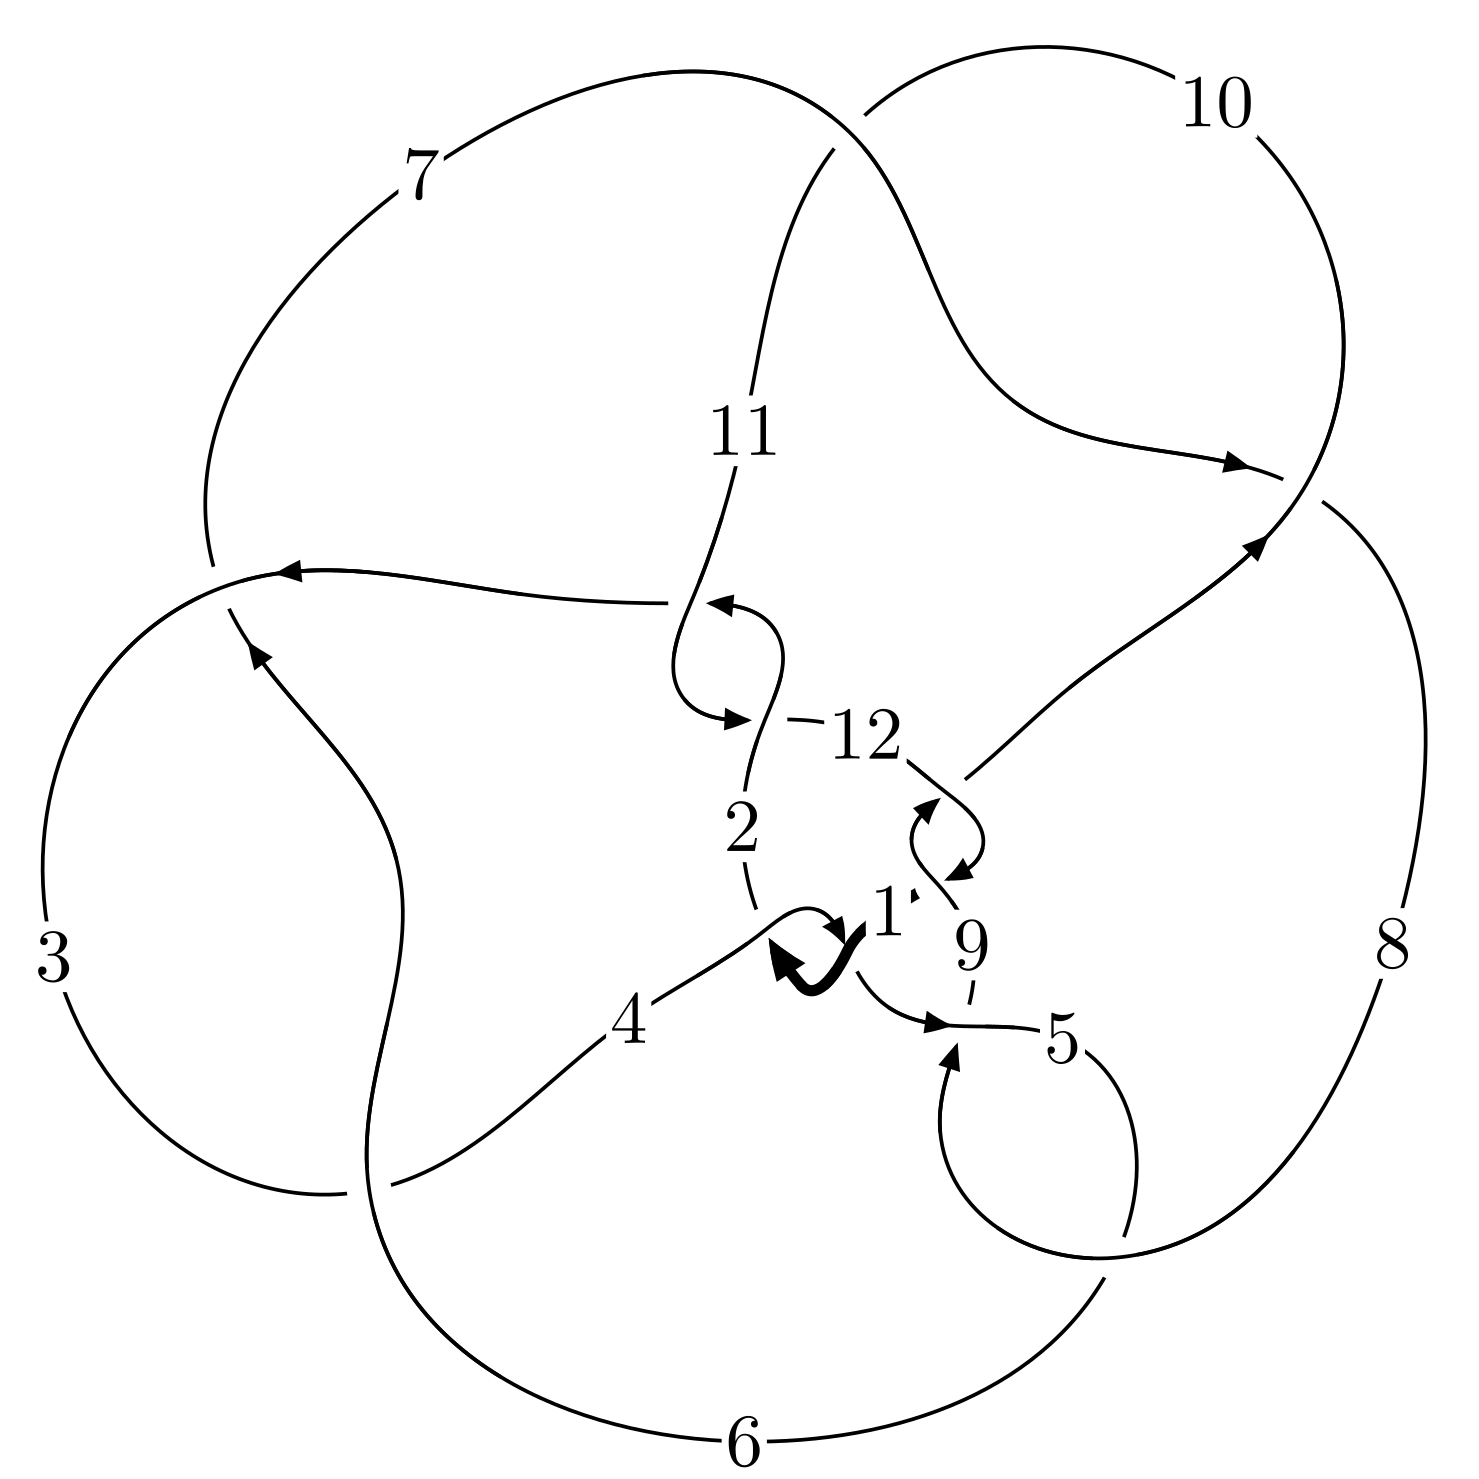
\includegraphics[width=112pt]{../../../GIT/diagram.site/diagram/png/2003_12a_1202.png}\\
\ \ \ A knot diagram\footnotemark}&
\allowdisplaybreaks
\textbf{Linearized knot diagam} \\
\cline{2-2}
 &
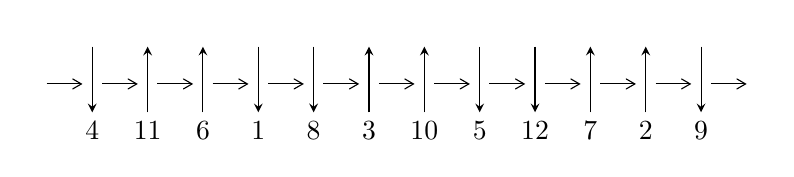
\begin{tikzpicture}[x=20pt, y=17pt]
	% nodes
	\node (C0) at (0, 0) {};
	\node (C1) at (1, 0) {};
	\node (C1U) at (1, +1) {};
	\node (C1D) at (1, -1) {4};

	\node (C2) at (2, 0) {};
	\node (C2U) at (2, +1) {};
	\node (C2D) at (2, -1) {11};

	\node (C3) at (3, 0) {};
	\node (C3U) at (3, +1) {};
	\node (C3D) at (3, -1) {6};

	\node (C4) at (4, 0) {};
	\node (C4U) at (4, +1) {};
	\node (C4D) at (4, -1) {1};

	\node (C5) at (5, 0) {};
	\node (C5U) at (5, +1) {};
	\node (C5D) at (5, -1) {8};

	\node (C6) at (6, 0) {};
	\node (C6U) at (6, +1) {};
	\node (C6D) at (6, -1) {3};

	\node (C7) at (7, 0) {};
	\node (C7U) at (7, +1) {};
	\node (C7D) at (7, -1) {10};

	\node (C8) at (8, 0) {};
	\node (C8U) at (8, +1) {};
	\node (C8D) at (8, -1) {5};

	\node (C9) at (9, 0) {};
	\node (C9U) at (9, +1) {};
	\node (C9D) at (9, -1) {12};

	\node (C10) at (10, 0) {};
	\node (C10U) at (10, +1) {};
	\node (C10D) at (10, -1) {7};

	\node (C11) at (11, 0) {};
	\node (C11U) at (11, +1) {};
	\node (C11D) at (11, -1) {2};

	\node (C12) at (12, 0) {};
	\node (C12U) at (12, +1) {};
	\node (C12D) at (12, -1) {9};
	\node (C13) at (13, 0) {};

	% arrows
	\draw[->,>={angle 60}]
	(C0) edge (C1) (C1) edge (C2) (C2) edge (C3) (C3) edge (C4) (C4) edge (C5) (C5) edge (C6) (C6) edge (C7) (C7) edge (C8) (C8) edge (C9) (C9) edge (C10) (C10) edge (C11) (C11) edge (C12) (C12) edge (C13) ;	\draw[->,>=stealth]
	(C1U) edge (C1D) (C2D) edge (C2U) (C3D) edge (C3U) (C4U) edge (C4D) (C5U) edge (C5D) (C6D) edge (C6U) (C7D) edge (C7U) (C8U) edge (C8D) (C9U) edge (C9D) (C10D) edge (C10U) (C11D) edge (C11U) (C12U) edge (C12D) ;
	\end{tikzpicture} \\
\hhline{~~} \\& 
\textbf{Solving Sequence} \\ \cline{2-2} 
 &
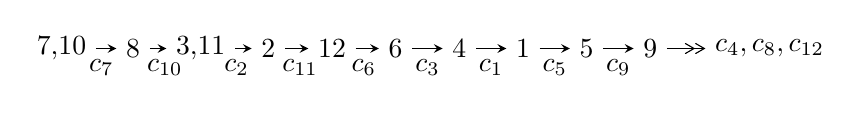
\begin{tikzpicture}[x=23pt, y=7pt]
	% node
	\node (A0) at (-1/8, 0) {7,10};
	\node (A1) at (1, 0) {8};
	\node (A2) at (33/16, 0) {3,11};
	\node (A3) at (25/8, 0) {2};
	\node (A4) at (33/8, 0) {12};
	\node (A5) at (41/8, 0) {6};
	\node (A6) at (49/8, 0) {4};
	\node (A7) at (57/8, 0) {1};
	\node (A8) at (65/8, 0) {5};
	\node (A9) at (73/8, 0) {9};
	\node (C1) at (1/2, -1) {$c_{7}$};
	\node (C2) at (3/2, -1) {$c_{10}$};
	\node (C3) at (21/8, -1) {$c_{2}$};
	\node (C4) at (29/8, -1) {$c_{11}$};
	\node (C5) at (37/8, -1) {$c_{6}$};
	\node (C6) at (45/8, -1) {$c_{3}$};
	\node (C7) at (53/8, -1) {$c_{1}$};
	\node (C8) at (61/8, -1) {$c_{5}$};
	\node (C9) at (69/8, -1) {$c_{9}$};
	\node (A10) at (11, 0) {$c_{4},c_{8},c_{12}$};

	% edge
	\draw[->,>=stealth]	
	(A0) edge (A1) (A1) edge (A2) (A2) edge (A3) (A3) edge (A4) (A4) edge (A5) (A5) edge (A6) (A6) edge (A7) (A7) edge (A8) (A8) edge (A9) ;
	\draw[->>,>={angle 60}]	
	(A9) edge (A10);
\end{tikzpicture} \\ 

\end{tabular} \\

\footnotetext{
The image of knot diagram is generated by the software ``\textbf{Draw programme}" developed by Andrew Bartholomew(\url{http://www.layer8.co.uk/maths/draw/index.htm\#Running-draw}), where we modified some parts for our purpose(\url{https://github.com/CATsTAILs/LinksPainter}).
}\phantom \\ \newline 
\centering \textbf{Ideals for irreducible components\footnotemark of $X_{\text{par}}$} 
 
\begin{align*}
I^u_{1}&=\langle 
b+u,\;a+u-1,\;u^8-3 u^7+8 u^6-11 u^5+12 u^4-7 u^3+2 u^2+1\rangle \\
I^u_{2}&=\langle 
b+u,\\
\phantom{I^u_{2}}&\phantom{= \langle  }5 u^{13}+8 u^{12}+37 u^{11}+36 u^{10}+87 u^9+50 u^8+68 u^7+14 u^6-24 u^5-10 u^4-31 u^3+14 u^2+4 a+31 u+8,\\
\phantom{I^u_{2}}&\phantom{= \langle  }u^{14}+2 u^{13}+8 u^{12}+10 u^{11}+20 u^{10}+16 u^9+17 u^8+6 u^7-4 u^6-6 u^5-7 u^4+6 u^2+4 u+1\rangle \\
I^u_{3}&=\langle 
2 u^{13}+3 u^{12}+14 u^{11}+13 u^{10}+30 u^9+17 u^8+16 u^7+4 u^6-20 u^5-4 u^4-14 u^3+3 u^2+4 b+12 u+5,\\
\phantom{I^u_{3}}&\phantom{= \langle  }2 u^{13}+3 u^{12}+14 u^{11}+13 u^{10}+30 u^9+17 u^8+16 u^7+4 u^6-20 u^5-4 u^4-14 u^3+3 u^2+4 a+12 u+1,\\
\phantom{I^u_{3}}&\phantom{= \langle  }u^{14}+2 u^{13}+8 u^{12}+10 u^{11}+20 u^{10}+16 u^9+17 u^8+6 u^7-4 u^6-6 u^5-7 u^4+6 u^2+4 u+1\rangle \\
I^u_{4}&=\langle 
150778247696 u^{13}-1269915907352 u^{12}+\cdots+29523131488 b-694243865440,\\
\phantom{I^u_{4}}&\phantom{= \langle  }-45565437328 u^{13}+456270050744 u^{12}+\cdots+59046262976 a+429363368096,\\
\phantom{I^u_{4}}&\phantom{= \langle  }16 u^{14}-152 u^{13}+\cdots-384 u+64\rangle \\
I^u_{5}&=\langle 
b+u,\;a+u+1,\;u^8+u^7+4 u^6+u^5+4 u^4- u^3+2 u^2+1\rangle \\
I^u_{6}&=\langle 
-4 u^{17} a-67 u^{17}+\cdots-4 a+48,\;u^{17} a+35 u^{17}+\cdots+14 a-83,\;u^{18}+3 u^{17}+\cdots-5 u+1\rangle \\
I^u_{7}&=\langle 
- u^5 a^3+u^5 a^2+\cdots+a+2,\;- u^5 a^3+u^5 a^2+\cdots- b- a,\\
\phantom{I^u_{7}}&\phantom{= \langle  }u^5 a^2+u^3 a^2+u^5- u^3 a- u^4- u^2 a+b u- a u- u^2- b+u+1,\\
\phantom{I^u_{7}}&\phantom{= \langle  }u^6 a^2+2 u^4 a^2+u^6- u^4 a- u^5+a^2 u^2- u^3 a+u^4- u^2 a-2 u^3- a u+u^2+1\rangle \\
\\
\end{align*}
\raggedright * 6 irreducible components of $\dim_{\mathbb{C}}=0$, with total 94 representations.\\
\raggedright * 1 irreducible components of $\dim_{\mathbb{C}}=1$ \\
\footnotetext{All coefficients of polynomials are rational numbers. But the coefficients are sometimes approximated in decimal forms when there is not enough margin.}
\newpage
\renewcommand{\arraystretch}{1}
\centering \section*{I. $I^u_{1}= \langle b+u,\;a+u-1,\;u^8-3 u^7+8 u^6-11 u^5+12 u^4-7 u^3+2 u^2+1 \rangle$}
\flushleft \textbf{(i) Arc colorings}\\
\begin{tabular}{m{7pt} m{180pt} m{7pt} m{180pt} }
\flushright $a_{7}=$&$\begin{pmatrix}1\\0\end{pmatrix}$ \\
\flushright $a_{10}=$&$\begin{pmatrix}0\\u\end{pmatrix}$ \\
\flushright $a_{8}=$&$\begin{pmatrix}1\\- u^2\end{pmatrix}$ \\
\flushright $a_{3}=$&$\begin{pmatrix}- u+1\\- u\end{pmatrix}$ \\
\flushright $a_{11}=$&$\begin{pmatrix}u\\u\end{pmatrix}$ \\
\flushright $a_{2}=$&$\begin{pmatrix}u^2- u+1\\u^2- u\end{pmatrix}$ \\
\flushright $a_{12}=$&$\begin{pmatrix}u^3- u^2+2 u\\u^3- u^2+u\end{pmatrix}$ \\
\flushright $a_{6}=$&$\begin{pmatrix}u^2- u+1\\u^2\end{pmatrix}$ \\
\flushright $a_{4}=$&$\begin{pmatrix}- u^3+u^2-2 u+1\\- u^3- u\end{pmatrix}$ \\
\flushright $a_{1}=$&$\begin{pmatrix}- u^7+2 u^6-5 u^5+5 u^4-5 u^3+3 u^2- u+1\\- u^7+u^6-3 u^5+u^4-2 u^3+u^2- u\end{pmatrix}$ \\
\flushright $a_{5}=$&$\begin{pmatrix}u^4- u^3+3 u^2- u+1\\- u^6+u^5-2 u^4+u^2\end{pmatrix}$ \\
\flushright $a_{9}=$&$\begin{pmatrix}u^7-2 u^6+5 u^5-4 u^4+4 u^3\\u^7-2 u^6+4 u^5-3 u^4+2 u^3+u\end{pmatrix}$\\&\end{tabular}
\flushleft \textbf{(ii) Obstruction class $= -1$}\\~\\
\flushleft \textbf{(iii) Cusp Shapes $= -3 u^7+3 u^6-6 u^5-6 u^4+12 u^3-15 u^2+9 u$}\\~\\
\newpage\renewcommand{\arraystretch}{1}
\flushleft \textbf{(iv) u-Polynomials at the component}\newline \\
\begin{tabular}{m{50pt}|m{274pt}}
Crossings & \hspace{64pt}u-Polynomials at each crossing \\
\hline $$\begin{aligned}c_{1},c_{4},c_{5}\\c_{8},c_{9},c_{12}\end{aligned}$$&$\begin{aligned}
&u^8-3 u^7+8 u^6-11 u^5+12 u^4-7 u^3+2 u^2+1
\end{aligned}$\\
\hline $$\begin{aligned}c_{2},c_{3},c_{6}\\c_{7},c_{10},c_{11}\end{aligned}$$&$\begin{aligned}
&u^8+3 u^7+8 u^6+11 u^5+12 u^4+7 u^3+2 u^2+1
\end{aligned}$\\
\hline
\end{tabular}\\~\\
\newpage\renewcommand{\arraystretch}{1}
\flushleft \textbf{(v) Riley Polynomials at the component}\newline \\
\begin{tabular}{m{50pt}|m{274pt}}
Crossings & \hspace{64pt}Riley Polynomials at each crossing \\
\hline $$\begin{aligned}c_{1},c_{2},c_{3}\\c_{4},c_{5},c_{6}\\c_{7},c_{8},c_{9}\\c_{10},c_{11},c_{12}\end{aligned}$$&$\begin{aligned}
&y^8+7 y^7+22 y^6+33 y^5+24 y^4+15 y^3+28 y^2+4 y+1
\end{aligned}$\\
\hline
\end{tabular}\\~\\
\newpage\flushleft \textbf{(vi) Complex Volumes and Cusp Shapes}
$$\begin{array}{c|c|c}  
\text{Solutions to }I^u_{1}& \I (\text{vol} + \sqrt{-1}CS) & \text{Cusp shape}\\
 \hline 
\begin{aligned}
u &= \phantom{-}0.802481 + 0.507921 I \\
a &= \phantom{-}0.197519 - 0.507921 I \\
b &= -0.802481 - 0.507921 I\end{aligned}
 & \phantom{-}9.81664 - 1.80153 I & \phantom{-}6.98214 - 1.70884 I \\ \hline\begin{aligned}
u &= \phantom{-}0.802481 - 0.507921 I \\
a &= \phantom{-}0.197519 + 0.507921 I \\
b &= -0.802481 + 0.507921 I\end{aligned}
 & \phantom{-}9.81664 + 1.80153 I & \phantom{-}6.98214 + 1.70884 I \\ \hline\begin{aligned}
u &= \phantom{-}0.36074 + 1.40947 I \\
a &= \phantom{-}0.63926 - 1.40947 I \\
b &= -0.36074 - 1.40947 I\end{aligned}
 & -9.81664 + 1.80153 I & -6.98214 + 1.70884 I \\ \hline\begin{aligned}
u &= \phantom{-}0.36074 - 1.40947 I \\
a &= \phantom{-}0.63926 + 1.40947 I \\
b &= -0.36074 + 1.40947 I\end{aligned}
 & -9.81664 - 1.80153 I & -6.98214 - 1.70884 I \\ \hline\begin{aligned}
u &= -0.252888 + 0.365077 I \\
a &= \phantom{-}1.252890 - 0.365077 I \\
b &= \phantom{-}0.252888 - 0.365077 I\end{aligned}
 & \phantom{-0.000000 } -1.13765 I & \phantom{-0.000000 -}0. + 6.26766 I \\ \hline\begin{aligned}
u &= -0.252888 - 0.365077 I \\
a &= \phantom{-}1.252890 + 0.365077 I \\
b &= \phantom{-}0.252888 + 0.365077 I\end{aligned}
 & \phantom{-0.000000 -}1.13765 I & \phantom{-0.000000 } 0. - 6.26766 I \\ \hline\begin{aligned}
u &= \phantom{-}0.58967 + 1.51917 I \\
a &= \phantom{-}0.41033 - 1.51917 I \\
b &= -0.58967 - 1.51917 I\end{aligned}
 & \phantom{-0.000000 -}18.0487 I & \phantom{-0.000000 } 0. - 8.38908 I \\ \hline\begin{aligned}
u &= \phantom{-}0.58967 - 1.51917 I \\
a &= \phantom{-}0.41033 + 1.51917 I \\
b &= -0.58967 + 1.51917 I\end{aligned}
 & \phantom{-0.000000 } -18.0487 I & \phantom{-0.000000 -}0. + 8.38908 I\\
 \hline 
 \end{array}$$\newpage\newpage\renewcommand{\arraystretch}{1}
\centering \section*{II. $I^u_{2}= \langle b+u,\;5 u^{13}+8 u^{12}+\cdots+4 a+8,\;u^{14}+2 u^{13}+\cdots+4 u+1 \rangle$}
\flushleft \textbf{(i) Arc colorings}\\
\begin{tabular}{m{7pt} m{180pt} m{7pt} m{180pt} }
\flushright $a_{7}=$&$\begin{pmatrix}1\\0\end{pmatrix}$ \\
\flushright $a_{10}=$&$\begin{pmatrix}0\\u\end{pmatrix}$ \\
\flushright $a_{8}=$&$\begin{pmatrix}1\\- u^2\end{pmatrix}$ \\
\flushright $a_{3}=$&$\begin{pmatrix}-\frac{5}{4} u^{13}-2 u^{12}+\cdots-\frac{31}{4} u-2\\- u\end{pmatrix}$ \\
\flushright $a_{11}=$&$\begin{pmatrix}u\\u\end{pmatrix}$ \\
\flushright $a_{2}=$&$\begin{pmatrix}-\frac{3}{2} u^{13}-\frac{5}{2} u^{12}+\cdots-\frac{17}{2} u-\frac{5}{2}\\-\frac{1}{4} u^{13}-\frac{1}{2} u^{12}+\cdots-\frac{7}{4} u-\frac{1}{2}\end{pmatrix}$ \\
\flushright $a_{12}=$&$\begin{pmatrix}u^{13}+\frac{3}{2} u^{12}+\cdots+5 u+2\\\frac{3}{16} u^{13}+\frac{1}{8} u^{12}+\cdots+\frac{31}{16} u+\frac{3}{4}\end{pmatrix}$ \\
\flushright $a_{6}=$&$\begin{pmatrix}-\frac{1}{2} u^{13}-\frac{3}{4} u^{12}+\cdots-3 u-\frac{1}{4}\\u^2\end{pmatrix}$ \\
\flushright $a_{4}=$&$\begin{pmatrix}-\frac{3}{2} u^{13}-\frac{5}{2} u^{12}+\cdots-\frac{19}{2} u-\frac{5}{2}\\- u^3- u\end{pmatrix}$ \\
\flushright $a_{1}=$&$\begin{pmatrix}-\frac{1}{2} u^{12}-\frac{1}{2} u^{11}+\cdots-4 u-\frac{3}{2}\\-\frac{3}{4} u^{13}-\frac{3}{2} u^{12}+\cdots-\frac{17}{4} u-\frac{3}{2}\end{pmatrix}$ \\
\flushright $a_{5}=$&$\begin{pmatrix}-\frac{1}{2} u^{13}- u^{12}+\cdots-\frac{7}{2} u-\frac{1}{2}\\-\frac{1}{2} u^{13}-\frac{3}{4} u^{12}+\cdots- u-\frac{1}{4}\end{pmatrix}$ \\
\flushright $a_{9}=$&$\begin{pmatrix}u^{13}+\frac{3}{2} u^{12}+\cdots+3 u+\frac{3}{2}\\-\frac{1}{4} u^{13}-\frac{1}{16} u^{12}+\cdots+u+\frac{3}{16}\end{pmatrix}$\\&\end{tabular}
\flushleft \textbf{(ii) Obstruction class $= -1$}\\~\\
\flushleft \textbf{(iii) Cusp Shapes $= \frac{71}{8} u^{13}+\frac{61}{4} u^{12}+\frac{541}{8} u^{11}+\frac{137}{2} u^{10}+\frac{1283}{8} u^9+\frac{175}{2} u^8+125 u^7+\frac{5}{4} u^6-\frac{79}{2} u^5-\frac{87}{2} u^4-\frac{381}{8} u^3+27 u^2+\frac{411}{8} u+\frac{39}{2}$}\\~\\
\newpage\renewcommand{\arraystretch}{1}
\flushleft \textbf{(iv) u-Polynomials at the component}\newline \\
\begin{tabular}{m{50pt}|m{274pt}}
Crossings & \hspace{64pt}u-Polynomials at each crossing \\
\hline $$\begin{aligned}c_{1},c_{4},c_{9}\\c_{12}\end{aligned}$$&$\begin{aligned}
&u^{14}+2 u^{13}+\cdots+4 u+1
\end{aligned}$\\
\hline $$\begin{aligned}c_{2},c_{11}\end{aligned}$$&$\begin{aligned}
&16(16 u^{14}+152 u^{13}+\cdots+384 u+64)
\end{aligned}$\\
\hline $$\begin{aligned}c_{3},c_{6},c_{7}\\c_{10}\end{aligned}$$&$\begin{aligned}
&u^{14}-2 u^{13}+\cdots-4 u+1
\end{aligned}$\\
\hline $$\begin{aligned}c_{5},c_{8}\end{aligned}$$&$\begin{aligned}
&16(16 u^{14}-152 u^{13}+\cdots-384 u+64)
\end{aligned}$\\
\hline
\end{tabular}\\~\\
\newpage\renewcommand{\arraystretch}{1}
\flushleft \textbf{(v) Riley Polynomials at the component}\newline \\
\begin{tabular}{m{50pt}|m{274pt}}
Crossings & \hspace{64pt}Riley Polynomials at each crossing \\
\hline $$\begin{aligned}c_{1},c_{3},c_{4}\\c_{6},c_{7},c_{9}\\c_{10},c_{12}\end{aligned}$$&$\begin{aligned}
&y^{14}+12 y^{13}+\cdots-4 y+1
\end{aligned}$\\
\hline $$\begin{aligned}c_{2},c_{5},c_{8}\\c_{11}\end{aligned}$$&$\begin{aligned}
&256(256 y^{14}+736 y^{13}+\cdots+22528 y+4096)
\end{aligned}$\\
\hline
\end{tabular}\\~\\
\newpage\flushleft \textbf{(vi) Complex Volumes and Cusp Shapes}
$$\begin{array}{c|c|c}  
\text{Solutions to }I^u_{2}& \I (\text{vol} + \sqrt{-1}CS) & \text{Cusp shape}\\
 \hline 
\begin{aligned}
u &= \phantom{-}0.735177 + 0.243598 I \\
a &= -0.31889 - 1.70839 I \\
b &= -0.735177 - 0.243598 I\end{aligned}
 & \phantom{-}8.49202 - 7.10507 I & \phantom{-}5.55614 + 2.56250 I \\ \hline\begin{aligned}
u &= \phantom{-}0.735177 - 0.243598 I \\
a &= -0.31889 + 1.70839 I \\
b &= -0.735177 + 0.243598 I\end{aligned}
 & \phantom{-}8.49202 + 7.10507 I & \phantom{-}5.55614 - 2.56250 I \\ \hline\begin{aligned}
u &= \phantom{-}0.330527 + 1.221190 I \\
a &= \phantom{-}0.11627 - 2.33392 I \\
b &= -0.330527 - 1.221190 I\end{aligned}
 & \phantom{-}5.35568 + 10.94750 I & \phantom{-}1.20768 - 7.19213 I \\ \hline\begin{aligned}
u &= \phantom{-}0.330527 - 1.221190 I \\
a &= \phantom{-}0.11627 + 2.33392 I \\
b &= -0.330527 + 1.221190 I\end{aligned}
 & \phantom{-}5.35568 - 10.94750 I & \phantom{-}1.20768 + 7.19213 I \\ \hline\begin{aligned}
u &= -0.104132 + 1.285370 I \\
a &= \phantom{-}0.14969 - 1.95386 I \\
b &= \phantom{-}0.104132 - 1.285370 I\end{aligned}
 & -4.77245 - 2.59879 I & -6.95245 + 3.73921 I \\ \hline\begin{aligned}
u &= -0.104132 - 1.285370 I \\
a &= \phantom{-}0.14969 + 1.95386 I \\
b &= \phantom{-}0.104132 + 1.285370 I\end{aligned}
 & -4.77245 + 2.59879 I & -6.95245 - 3.73921 I \\ \hline\begin{aligned}
u &= -0.672210 + 0.160128 I \\
a &= -0.586673 + 0.704036 I \\
b &= \phantom{-}0.672210 - 0.160128 I\end{aligned}
 & \phantom{-}4.77245 - 2.59879 I & \phantom{-}6.95245 + 3.73921 I \\ \hline\begin{aligned}
u &= -0.672210 - 0.160128 I \\
a &= -0.586673 - 0.704036 I \\
b &= \phantom{-}0.672210 + 0.160128 I\end{aligned}
 & \phantom{-}4.77245 + 2.59879 I & \phantom{-}6.95245 - 3.73921 I \\ \hline\begin{aligned}
u &= -0.44398 + 1.43884 I \\
a &= -0.70423 - 1.58491 I \\
b &= \phantom{-}0.44398 - 1.43884 I\end{aligned}
 & -5.35568 - 10.94750 I & -1.20768 + 7.19213 I \\ \hline\begin{aligned}
u &= -0.44398 - 1.43884 I \\
a &= -0.70423 + 1.58491 I \\
b &= \phantom{-}0.44398 + 1.43884 I\end{aligned}
 & -5.35568 + 10.94750 I & -1.20768 - 7.19213 I\\
 \hline 
 \end{array}$$\newpage$$\begin{array}{c|c|c}  
\text{Solutions to }I^u_{2}& \I (\text{vol} + \sqrt{-1}CS) & \text{Cusp shape}\\
 \hline 
\begin{aligned}
u &= -0.362798 + 0.314516 I \\
a &= \phantom{-}1.21504 - 0.98313 I \\
b &= \phantom{-}0.362798 - 0.314516 I\end{aligned}
 & \phantom{-0.000000 } -1.12378 I & \phantom{-0.000000 -}0. + 6.09178 I \\ \hline\begin{aligned}
u &= -0.362798 - 0.314516 I \\
a &= \phantom{-}1.21504 + 0.98313 I \\
b &= \phantom{-}0.362798 + 0.314516 I\end{aligned}
 & \phantom{-0.000000 -}1.12378 I & \phantom{-0.000000 } 0. - 6.09178 I \\ \hline\begin{aligned}
u &= -0.48258 + 1.50879 I \\
a &= -0.37121 - 1.49894 I \\
b &= \phantom{-}0.48258 - 1.50879 I\end{aligned}
 & -8.49202 - 7.10507 I & -5.55614 + 2.56250 I \\ \hline\begin{aligned}
u &= -0.48258 - 1.50879 I \\
a &= -0.37121 + 1.49894 I \\
b &= \phantom{-}0.48258 + 1.50879 I\end{aligned}
 & -8.49202 + 7.10507 I & -5.55614 - 2.56250 I\\
 \hline 
 \end{array}$$\newpage\newpage\renewcommand{\arraystretch}{1}
\centering \section*{III. $I^u_{3}= \langle 2 u^{13}+3 u^{12}+\cdots+4 b+5,\;2 u^{13}+3 u^{12}+\cdots+4 a+1,\;u^{14}+2 u^{13}+\cdots+4 u+1 \rangle$}
\flushleft \textbf{(i) Arc colorings}\\
\begin{tabular}{m{7pt} m{180pt} m{7pt} m{180pt} }
\flushright $a_{7}=$&$\begin{pmatrix}1\\0\end{pmatrix}$ \\
\flushright $a_{10}=$&$\begin{pmatrix}0\\u\end{pmatrix}$ \\
\flushright $a_{8}=$&$\begin{pmatrix}1\\- u^2\end{pmatrix}$ \\
\flushright $a_{3}=$&$\begin{pmatrix}-\frac{1}{2} u^{13}-\frac{3}{4} u^{12}+\cdots-3 u-\frac{1}{4}\\-\frac{1}{2} u^{13}-\frac{3}{4} u^{12}+\cdots-3 u-\frac{5}{4}\end{pmatrix}$ \\
\flushright $a_{11}=$&$\begin{pmatrix}u\\u\end{pmatrix}$ \\
\flushright $a_{2}=$&$\begin{pmatrix}-\frac{1}{2} u^{13}-\frac{3}{4} u^{12}+\cdots-3 u-\frac{1}{4}\\-\frac{1}{2} u^{13}-\frac{3}{4} u^{12}+\cdots-3 u-\frac{5}{4}\end{pmatrix}$ \\
\flushright $a_{12}=$&$\begin{pmatrix}\frac{1}{4} u^{13}+\frac{1}{2} u^{12}+\cdots+\frac{11}{4} u+\frac{1}{2}\\\frac{1}{4} u^{13}+\frac{1}{2} u^{12}+\cdots+\frac{7}{4} u+\frac{1}{2}\end{pmatrix}$ \\
\flushright $a_{6}=$&$\begin{pmatrix}-\frac{3}{4} u^{13}-\frac{21}{16} u^{12}+\cdots-5 u-\frac{17}{16}\\-\frac{1}{4} u^{13}-\frac{9}{16} u^{12}+\cdots-2 u-\frac{13}{16}\end{pmatrix}$ \\
\flushright $a_{4}=$&$\begin{pmatrix}-0.812500 u^{13}-1.54688 u^{12}+\cdots-4.25000 u-0.984375\\-0.0625000 u^{13}-0.234375 u^{12}+\cdots+0.750000 u+0.0781250\end{pmatrix}$ \\
\flushright $a_{1}=$&$\begin{pmatrix}0.421875 u^{13}+1.03125 u^{12}+\cdots+2.23438 u+1.18750\\0.609375 u^{13}+1.65625 u^{12}+\cdots+3.17188 u+0.937500\end{pmatrix}$ \\
\flushright $a_{5}=$&$\begin{pmatrix}-\frac{5}{4} u^{13}-\frac{29}{16} u^{12}+\cdots-7 u-\frac{33}{16}\\\frac{1}{4} u^{13}+\frac{7}{16} u^{12}+\cdots-\frac{1}{2} u-\frac{5}{16}\end{pmatrix}$ \\
\flushright $a_{9}=$&$\begin{pmatrix}-0.687500 u^{13}-1.12500 u^{12}+\cdots-3.43750 u-0.750000\\-\frac{7}{16} u^{13}-\frac{9}{8} u^{12}+\cdots-\frac{35}{16} u-\frac{3}{4}\end{pmatrix}$\\&\end{tabular}
\flushleft \textbf{(ii) Obstruction class $= -1$}\\~\\
\flushleft \textbf{(iii) Cusp Shapes $= \frac{71}{8} u^{13}+\frac{61}{4} u^{12}+\frac{541}{8} u^{11}+\frac{137}{2} u^{10}+\frac{1283}{8} u^9+\frac{175}{2} u^8+125 u^7+\frac{5}{4} u^6-\frac{79}{2} u^5-\frac{87}{2} u^4-\frac{381}{8} u^3+27 u^2+\frac{411}{8} u+\frac{39}{2}$}\\~\\
\newpage\renewcommand{\arraystretch}{1}
\flushleft \textbf{(iv) u-Polynomials at the component}\newline \\
\begin{tabular}{m{50pt}|m{274pt}}
Crossings & \hspace{64pt}u-Polynomials at each crossing \\
\hline $$\begin{aligned}c_{1},c_{4},c_{5}\\c_{8}\end{aligned}$$&$\begin{aligned}
&u^{14}+2 u^{13}+\cdots+4 u+1
\end{aligned}$\\
\hline $$\begin{aligned}c_{2},c_{7},c_{10}\\c_{11}\end{aligned}$$&$\begin{aligned}
&u^{14}-2 u^{13}+\cdots-4 u+1
\end{aligned}$\\
\hline $$\begin{aligned}c_{3},c_{6}\end{aligned}$$&$\begin{aligned}
&16(16 u^{14}+152 u^{13}+\cdots+384 u+64)
\end{aligned}$\\
\hline $$\begin{aligned}c_{9},c_{12}\end{aligned}$$&$\begin{aligned}
&16(16 u^{14}-152 u^{13}+\cdots-384 u+64)
\end{aligned}$\\
\hline
\end{tabular}\\~\\
\newpage\renewcommand{\arraystretch}{1}
\flushleft \textbf{(v) Riley Polynomials at the component}\newline \\
\begin{tabular}{m{50pt}|m{274pt}}
Crossings & \hspace{64pt}Riley Polynomials at each crossing \\
\hline $$\begin{aligned}c_{1},c_{2},c_{4}\\c_{5},c_{7},c_{8}\\c_{10},c_{11}\end{aligned}$$&$\begin{aligned}
&y^{14}+12 y^{13}+\cdots-4 y+1
\end{aligned}$\\
\hline $$\begin{aligned}c_{3},c_{6},c_{9}\\c_{12}\end{aligned}$$&$\begin{aligned}
&256(256 y^{14}+736 y^{13}+\cdots+22528 y+4096)
\end{aligned}$\\
\hline
\end{tabular}\\~\\
\newpage\flushleft \textbf{(vi) Complex Volumes and Cusp Shapes}
$$\begin{array}{c|c|c}  
\text{Solutions to }I^u_{3}& \I (\text{vol} + \sqrt{-1}CS) & \text{Cusp shape}\\
 \hline 
\begin{aligned}
u &= \phantom{-}0.735177 + 0.243598 I \\
a &= \phantom{-}0.337138 + 0.975478 I \\
b &= -0.662862 + 0.975478 I\end{aligned}
 & \phantom{-}8.49202 - 7.10507 I & \phantom{-}5.55614 + 2.56250 I \\ \hline\begin{aligned}
u &= \phantom{-}0.735177 - 0.243598 I \\
a &= \phantom{-}0.337138 - 0.975478 I \\
b &= -0.662862 - 0.975478 I\end{aligned}
 & \phantom{-}8.49202 + 7.10507 I & \phantom{-}5.55614 - 2.56250 I \\ \hline\begin{aligned}
u &= \phantom{-}0.330527 + 1.221190 I \\
a &= -0.506537 - 0.177835 I \\
b &= -1.50654 - 0.17783 I\end{aligned}
 & \phantom{-}5.35568 + 10.94750 I & \phantom{-}1.20768 - 7.19213 I \\ \hline\begin{aligned}
u &= \phantom{-}0.330527 - 1.221190 I \\
a &= -0.506537 + 0.177835 I \\
b &= -1.50654 + 0.17783 I\end{aligned}
 & \phantom{-}5.35568 - 10.94750 I & \phantom{-}1.20768 + 7.19213 I \\ \hline\begin{aligned}
u &= -0.104132 + 1.285370 I \\
a &= \phantom{-}0.145481 - 0.128174 I \\
b &= -0.854519 - 0.128174 I\end{aligned}
 & -4.77245 - 2.59879 I & -6.95245 + 3.73921 I \\ \hline\begin{aligned}
u &= -0.104132 - 1.285370 I \\
a &= \phantom{-}0.145481 + 0.128174 I \\
b &= -0.854519 + 0.128174 I\end{aligned}
 & -4.77245 + 2.59879 I & -6.95245 - 3.73921 I \\ \hline\begin{aligned}
u &= -0.672210 + 0.160128 I \\
a &= \phantom{-}0.292144 + 0.782483 I \\
b &= -0.707856 + 0.782483 I\end{aligned}
 & \phantom{-}4.77245 - 2.59879 I & \phantom{-}6.95245 + 3.73921 I \\ \hline\begin{aligned}
u &= -0.672210 - 0.160128 I \\
a &= \phantom{-}0.292144 - 0.782483 I \\
b &= -0.707856 - 0.782483 I\end{aligned}
 & \phantom{-}4.77245 + 2.59879 I & \phantom{-}6.95245 - 3.73921 I \\ \hline\begin{aligned}
u &= -0.44398 + 1.43884 I \\
a &= \phantom{-}0.28005 + 1.58724 I \\
b &= -0.71995 + 1.58724 I\end{aligned}
 & -5.35568 - 10.94750 I & -1.20768 + 7.19213 I \\ \hline\begin{aligned}
u &= -0.44398 - 1.43884 I \\
a &= \phantom{-}0.28005 - 1.58724 I \\
b &= -0.71995 - 1.58724 I\end{aligned}
 & -5.35568 + 10.94750 I & -1.20768 - 7.19213 I\\
 \hline 
 \end{array}$$\newpage$$\begin{array}{c|c|c}  
\text{Solutions to }I^u_{3}& \I (\text{vol} + \sqrt{-1}CS) & \text{Cusp shape}\\
 \hline 
\begin{aligned}
u &= -0.362798 + 0.314516 I \\
a &= \phantom{-}1.098900 - 0.510617 I \\
b &= \phantom{-}0.098902 - 0.510617 I\end{aligned}
 & \phantom{-0.000000 } -1.12378 I & \phantom{-0.000000 -}0. + 6.09178 I \\ \hline\begin{aligned}
u &= -0.362798 - 0.314516 I \\
a &= \phantom{-}1.098900 + 0.510617 I \\
b &= \phantom{-}0.098902 + 0.510617 I\end{aligned}
 & \phantom{-0.000000 -}1.12378 I & \phantom{-0.000000 } 0. - 6.09178 I \\ \hline\begin{aligned}
u &= -0.48258 + 1.50879 I \\
a &= \phantom{-}0.60282 + 1.29294 I \\
b &= -0.397177 + 1.292940 I\end{aligned}
 & -8.49202 - 7.10507 I & -5.55614 + 2.56250 I \\ \hline\begin{aligned}
u &= -0.48258 - 1.50879 I \\
a &= \phantom{-}0.60282 - 1.29294 I \\
b &= -0.397177 - 1.292940 I\end{aligned}
 & -8.49202 + 7.10507 I & -5.55614 - 2.56250 I\\
 \hline 
 \end{array}$$\newpage\newpage\renewcommand{\arraystretch}{1}
\centering \section*{IV. $I^u_{4}= \langle 1.51\times10^{11} u^{13}-1.27\times10^{12} u^{12}+\cdots+2.95\times10^{10} b-6.94\times10^{11},\;-4.56\times10^{10} u^{13}+4.56\times10^{11} u^{12}+\cdots+5.90\times10^{10} a+4.29\times10^{11},\;16 u^{14}-152 u^{13}+\cdots-384 u+64 \rangle$}
\flushleft \textbf{(i) Arc colorings}\\
\begin{tabular}{m{7pt} m{180pt} m{7pt} m{180pt} }
\flushright $a_{7}=$&$\begin{pmatrix}1\\0\end{pmatrix}$ \\
\flushright $a_{10}=$&$\begin{pmatrix}0\\u\end{pmatrix}$ \\
\flushright $a_{8}=$&$\begin{pmatrix}1\\- u^2\end{pmatrix}$ \\
\flushright $a_{3}=$&$\begin{pmatrix}0.771690 u^{13}-7.72733 u^{12}+\cdots+36.3451 u-7.27164\\-5.10712 u^{13}+43.0143 u^{12}+\cdots-110.305 u+23.5153\end{pmatrix}$ \\
\flushright $a_{11}=$&$\begin{pmatrix}u\\u\end{pmatrix}$ \\
\flushright $a_{2}=$&$\begin{pmatrix}6.27509 u^{13}-53.7103 u^{12}+\cdots+135.401 u-27.7001\\0.396272 u^{13}-2.96866 u^{12}+\cdots-11.2489 u+3.08676\end{pmatrix}$ \\
\flushright $a_{12}=$&$\begin{pmatrix}-0.433597 u^{13}+3.07351 u^{12}+\cdots+9.75173 u-3.28454\\-1.39433 u^{13}+13.2245 u^{12}+\cdots-39.2531 u+7.93893\end{pmatrix}$ \\
\flushright $a_{6}=$&$\begin{pmatrix}-1.98473 u^{13}+17.4606 u^{12}+\cdots-37.1706 u+8.38054\\-1.02400 u^{13}+7.30966 u^{12}+\cdots+11.8341 u-3.84294\end{pmatrix}$ \\
\flushright $a_{4}=$&$\begin{pmatrix}-6.45812 u^{13}+53.4349 u^{12}+\cdots-113.519 u+23.9546\\5.19125 u^{13}-46.5395 u^{12}+\cdots+130.406 u-26.1690\end{pmatrix}$ \\
\flushright $a_{1}=$&$\begin{pmatrix}2.29549 u^{13}-18.6841 u^{12}+\cdots+22.4712 u-3.09596\\1.93780 u^{13}-17.1761 u^{12}+\cdots+35.1477 u-7.07687\end{pmatrix}$ \\
\flushright $a_{5}=$&$\begin{pmatrix}-3.03039 u^{13}+26.1775 u^{12}+\cdots-50.8615 u+10.1149\\0.216231 u^{13}-3.35036 u^{12}+\cdots+36.8578 u-8.71066\end{pmatrix}$ \\
\flushright $a_{9}=$&$\begin{pmatrix}0.379426 u^{13}-2.77238 u^{12}+\cdots-1.09120 u+0.400513\\-0.177226 u^{13}+1.36624 u^{12}+\cdots-8.94746 u+1.81095\end{pmatrix}$\\&\end{tabular}
\flushleft \textbf{(ii) Obstruction class $= -1$}\\~\\
\flushleft \textbf{(iii) Cusp Shapes $= \frac{22971118306}{922597859} u^{13}-\frac{205737218319}{922597859} u^{12}+\cdots+\frac{620526036416}{922597859} u-\frac{129937751014}{922597859}$}\\~\\
\newpage\renewcommand{\arraystretch}{1}
\flushleft \textbf{(iv) u-Polynomials at the component}\newline \\
\begin{tabular}{m{50pt}|m{274pt}}
Crossings & \hspace{64pt}u-Polynomials at each crossing \\
\hline $$\begin{aligned}c_{1},c_{4}\end{aligned}$$&$\begin{aligned}
&16(16 u^{14}-152 u^{13}+\cdots-384 u+64)
\end{aligned}$\\
\hline $$\begin{aligned}c_{2},c_{3},c_{6}\\c_{11}\end{aligned}$$&$\begin{aligned}
&u^{14}-2 u^{13}+\cdots-4 u+1
\end{aligned}$\\
\hline $$\begin{aligned}c_{5},c_{8},c_{9}\\c_{12}\end{aligned}$$&$\begin{aligned}
&u^{14}+2 u^{13}+\cdots+4 u+1
\end{aligned}$\\
\hline $$\begin{aligned}c_{7},c_{10}\end{aligned}$$&$\begin{aligned}
&16(16 u^{14}+152 u^{13}+\cdots+384 u+64)
\end{aligned}$\\
\hline
\end{tabular}\\~\\
\newpage\renewcommand{\arraystretch}{1}
\flushleft \textbf{(v) Riley Polynomials at the component}\newline \\
\begin{tabular}{m{50pt}|m{274pt}}
Crossings & \hspace{64pt}Riley Polynomials at each crossing \\
\hline $$\begin{aligned}c_{1},c_{4},c_{7}\\c_{10}\end{aligned}$$&$\begin{aligned}
&256(256 y^{14}+736 y^{13}+\cdots+22528 y+4096)
\end{aligned}$\\
\hline $$\begin{aligned}c_{2},c_{3},c_{5}\\c_{6},c_{8},c_{9}\\c_{11},c_{12}\end{aligned}$$&$\begin{aligned}
&y^{14}+12 y^{13}+\cdots-4 y+1
\end{aligned}$\\
\hline
\end{tabular}\\~\\
\newpage\flushleft \textbf{(vi) Complex Volumes and Cusp Shapes}
$$\begin{array}{c|c|c}  
\text{Solutions to }I^u_{4}& \I (\text{vol} + \sqrt{-1}CS) & \text{Cusp shape}\\
 \hline 
\begin{aligned}
u &= \phantom{-}0.707856 + 0.782483 I \\
a &= \phantom{-}0.132280 + 0.530765 I \\
b &= \phantom{-}0.672210 + 0.160128 I\end{aligned}
 & \phantom{-}4.77245 + 2.59879 I & \phantom{-}6.95245 - 3.73921 I \\ \hline\begin{aligned}
u &= \phantom{-}0.707856 - 0.782483 I \\
a &= \phantom{-}0.132280 - 0.530765 I \\
b &= \phantom{-}0.672210 - 0.160128 I\end{aligned}
 & \phantom{-}4.77245 - 2.59879 I & \phantom{-}6.95245 + 3.73921 I \\ \hline\begin{aligned}
u &= \phantom{-}0.854519 + 0.128174 I \\
a &= \phantom{-}0.205611 + 0.203611 I \\
b &= \phantom{-}0.104132 - 1.285370 I\end{aligned}
 & -4.77245 - 2.59879 I & -6.95245 + 3.73921 I \\ \hline\begin{aligned}
u &= \phantom{-}0.854519 - 0.128174 I \\
a &= \phantom{-}0.205611 - 0.203611 I \\
b &= \phantom{-}0.104132 + 1.285370 I\end{aligned}
 & -4.77245 + 2.59879 I & -6.95245 - 3.73921 I \\ \hline\begin{aligned}
u &= \phantom{-}0.662862 + 0.975478 I \\
a &= -0.555661 - 0.388074 I \\
b &= -0.735177 + 0.243598 I\end{aligned}
 & \phantom{-}8.49202 + 7.10507 I & \phantom{-}5.55614 - 2.56250 I \\ \hline\begin{aligned}
u &= \phantom{-}0.662862 - 0.975478 I \\
a &= -0.555661 + 0.388074 I \\
b &= -0.735177 - 0.243598 I\end{aligned}
 & \phantom{-}8.49202 - 7.10507 I & \phantom{-}5.55614 + 2.56250 I \\ \hline\begin{aligned}
u &= \phantom{-}0.397177 + 1.292940 I \\
a &= -0.68850 + 1.52229 I \\
b &= \phantom{-}0.48258 + 1.50879 I\end{aligned}
 & -8.49202 + 7.10507 I & -5.55614 - 2.56250 I \\ \hline\begin{aligned}
u &= \phantom{-}0.397177 - 1.292940 I \\
a &= -0.68850 - 1.52229 I \\
b &= \phantom{-}0.48258 - 1.50879 I\end{aligned}
 & -8.49202 - 7.10507 I & -5.55614 + 2.56250 I \\ \hline\begin{aligned}
u &= -0.098902 + 0.510617 I \\
a &= \phantom{-}1.089120 + 0.255309 I \\
b &= \phantom{-}0.362798 - 0.314516 I\end{aligned}
 & \phantom{-0.000000 } -1.12378 I & \phantom{-0.000000 -}0. + 6.09178 I \\ \hline\begin{aligned}
u &= -0.098902 - 0.510617 I \\
a &= \phantom{-}1.089120 - 0.255309 I \\
b &= \phantom{-}0.362798 + 0.314516 I\end{aligned}
 & \phantom{-0.000000 -}1.12378 I & \phantom{-0.000000 } 0. - 6.09178 I\\
 \hline 
 \end{array}$$\newpage$$\begin{array}{c|c|c}  
\text{Solutions to }I^u_{4}& \I (\text{vol} + \sqrt{-1}CS) & \text{Cusp shape}\\
 \hline 
\begin{aligned}
u &= \phantom{-}1.50654 + 0.17783 I \\
a &= -0.019777 - 0.447277 I \\
b &= -0.330527 - 1.221190 I\end{aligned}
 & \phantom{-}5.35568 + 10.94750 I & \phantom{-}1.20768 - 7.19213 I \\ \hline\begin{aligned}
u &= \phantom{-}1.50654 - 0.17783 I \\
a &= -0.019777 + 0.447277 I \\
b &= -0.330527 + 1.221190 I\end{aligned}
 & \phantom{-}5.35568 - 10.94750 I & \phantom{-}1.20768 + 7.19213 I \\ \hline\begin{aligned}
u &= \phantom{-}0.71995 + 1.58724 I \\
a &= -0.413070 + 1.329820 I \\
b &= \phantom{-}0.44398 + 1.43884 I\end{aligned}
 & -5.35568 + 10.94750 I & -1.20768 - 7.19213 I \\ \hline\begin{aligned}
u &= \phantom{-}0.71995 - 1.58724 I \\
a &= -0.413070 - 1.329820 I \\
b &= \phantom{-}0.44398 - 1.43884 I\end{aligned}
 & -5.35568 - 10.94750 I & -1.20768 + 7.19213 I\\
 \hline 
 \end{array}$$\newpage\newpage\renewcommand{\arraystretch}{1}
\centering \section*{V. $I^u_{5}= \langle b+u,\;a+u+1,\;u^8+u^7+4 u^6+u^5+4 u^4- u^3+2 u^2+1 \rangle$}
\flushleft \textbf{(i) Arc colorings}\\
\begin{tabular}{m{7pt} m{180pt} m{7pt} m{180pt} }
\flushright $a_{7}=$&$\begin{pmatrix}1\\0\end{pmatrix}$ \\
\flushright $a_{10}=$&$\begin{pmatrix}0\\u\end{pmatrix}$ \\
\flushright $a_{8}=$&$\begin{pmatrix}1\\- u^2\end{pmatrix}$ \\
\flushright $a_{3}=$&$\begin{pmatrix}- u-1\\- u\end{pmatrix}$ \\
\flushright $a_{11}=$&$\begin{pmatrix}u\\u\end{pmatrix}$ \\
\flushright $a_{2}=$&$\begin{pmatrix}- u^2- u-1\\- u^2- u\end{pmatrix}$ \\
\flushright $a_{12}=$&$\begin{pmatrix}u^3+u^2+2 u\\u^3+u^2+u\end{pmatrix}$ \\
\flushright $a_{6}=$&$\begin{pmatrix}u^2+u+1\\u^2\end{pmatrix}$ \\
\flushright $a_{4}=$&$\begin{pmatrix}- u^3- u^2-2 u-1\\- u^3- u\end{pmatrix}$ \\
\flushright $a_{1}=$&$\begin{pmatrix}- u^7-2 u^6-5 u^5-5 u^4-5 u^3-3 u^2- u-1\\- u^7- u^6-3 u^5- u^4-2 u^3- u^2- u\end{pmatrix}$ \\
\flushright $a_{5}=$&$\begin{pmatrix}u^4+u^3+3 u^2+u+1\\- u^6- u^5-2 u^4+u^2\end{pmatrix}$ \\
\flushright $a_{9}=$&$\begin{pmatrix}u^7+2 u^6+5 u^5+4 u^4+4 u^3\\u^7+2 u^6+4 u^5+3 u^4+2 u^3+u\end{pmatrix}$\\&\end{tabular}
\flushleft \textbf{(ii) Obstruction class $= 1$}\\~\\
\flushleft \textbf{(iii) Cusp Shapes $= 3 u^7-3 u^6+6 u^5-18 u^4+6 u^3-21 u^2+9 u-6$}\\~\\
\newpage\renewcommand{\arraystretch}{1}
\flushleft \textbf{(iv) u-Polynomials at the component}\newline \\
\begin{tabular}{m{50pt}|m{274pt}}
Crossings & \hspace{64pt}u-Polynomials at each crossing \\
\hline $$\begin{aligned}c_{1},c_{2},c_{5}\\c_{6},c_{9},c_{10}\end{aligned}$$&$\begin{aligned}
&u^8- u^7+4 u^6- u^5+4 u^4+u^3+2 u^2+1
\end{aligned}$\\
\hline $$\begin{aligned}c_{3},c_{4},c_{7}\\c_{8},c_{11},c_{12}\end{aligned}$$&$\begin{aligned}
&u^8+u^7+4 u^6+u^5+4 u^4- u^3+2 u^2+1
\end{aligned}$\\
\hline
\end{tabular}\\~\\
\newpage\renewcommand{\arraystretch}{1}
\flushleft \textbf{(v) Riley Polynomials at the component}\newline \\
\begin{tabular}{m{50pt}|m{274pt}}
Crossings & \hspace{64pt}Riley Polynomials at each crossing \\
\hline $$\begin{aligned}c_{1},c_{2},c_{3}\\c_{4},c_{5},c_{6}\\c_{7},c_{8},c_{9}\\c_{10},c_{11},c_{12}\end{aligned}$$&$\begin{aligned}
&y^8+7 y^7+22 y^6+37 y^5+36 y^4+23 y^3+12 y^2+4 y+1
\end{aligned}$\\
\hline
\end{tabular}\\~\\
\newpage\flushleft \textbf{(vi) Complex Volumes and Cusp Shapes}
$$\begin{array}{c|c|c}  
\text{Solutions to }I^u_{5}& \I (\text{vol} + \sqrt{-1}CS) & \text{Cusp shape}\\
 \hline 
\begin{aligned}
u &= -0.200786 + 1.204120 I \\
a &= -0.79921 - 1.20412 I \\
b &= \phantom{-}0.200786 - 1.204120 I\end{aligned}
 & \phantom{-0.000000 } -1.61656 I & \phantom{-0.000000 -}     -6
0. 10   + 1.306426 I \\ \hline\begin{aligned}
u &= -0.200786 - 1.204120 I \\
a &= -0.79921 + 1.20412 I \\
b &= \phantom{-}0.200786 + 1.204120 I\end{aligned}
 & \phantom{-0.000000 -}1.61656 I & \phantom{-0.000000 }      -6
0. 10   - 1.306426 I \\ \hline\begin{aligned}
u &= \phantom{-}0.537476 + 0.510510 I \\
a &= -1.53748 - 0.51051 I \\
b &= -0.537476 - 0.510510 I\end{aligned}
 & \phantom{-}7.30226 + 8.49334 I & \phantom{-}1.28328 - 6.26325 I \\ \hline\begin{aligned}
u &= \phantom{-}0.537476 - 0.510510 I \\
a &= -1.53748 + 0.51051 I \\
b &= -0.537476 + 0.510510 I\end{aligned}
 & \phantom{-}7.30226 - 8.49334 I & \phantom{-}1.28328 + 6.26325 I \\ \hline\begin{aligned}
u &= -0.327893 + 0.646046 I \\
a &= -0.672107 - 0.646046 I \\
b &= \phantom{-}0.327893 - 0.646046 I\end{aligned}
 & \phantom{-0.000000 } -2.71955 I & \phantom{-0.000000 -}0. + 9.22661 I \\ \hline\begin{aligned}
u &= -0.327893 - 0.646046 I \\
a &= -0.672107 + 0.646046 I \\
b &= \phantom{-}0.327893 + 0.646046 I\end{aligned}
 & \phantom{-0.000000 -}2.71955 I & \phantom{-0.000000 } 0. - 9.22661 I \\ \hline\begin{aligned}
u &= -0.50880 + 1.43795 I \\
a &= -0.49120 - 1.43795 I \\
b &= \phantom{-}0.50880 - 1.43795 I\end{aligned}
 & -7.30226 - 8.49334 I & -1.28328 + 6.26325 I \\ \hline\begin{aligned}
u &= -0.50880 - 1.43795 I \\
a &= -0.49120 + 1.43795 I \\
b &= \phantom{-}0.50880 + 1.43795 I\end{aligned}
 & -7.30226 + 8.49334 I & -1.28328 - 6.26325 I\\
 \hline 
 \end{array}$$\newpage\newpage\renewcommand{\arraystretch}{1}
\centering \section*{VI. $I^u_{6}= \langle -4 u^{17} a-67 u^{17}+\cdots-4 a+48,\;u^{17} a+35 u^{17}+\cdots+14 a-83,\;u^{18}+3 u^{17}+\cdots-5 u+1 \rangle$}
\flushleft \textbf{(i) Arc colorings}\\
\begin{tabular}{m{7pt} m{180pt} m{7pt} m{180pt} }
\flushright $a_{7}=$&$\begin{pmatrix}1\\0\end{pmatrix}$ \\
\flushright $a_{10}=$&$\begin{pmatrix}0\\u\end{pmatrix}$ \\
\flushright $a_{8}=$&$\begin{pmatrix}1\\- u^2\end{pmatrix}$ \\
\flushright $a_{3}=$&$\begin{pmatrix}a\\0.0434783 a u^{17}+0.728261 u^{17}+\cdots+0.0434783 a-0.521739\end{pmatrix}$ \\
\flushright $a_{11}=$&$\begin{pmatrix}u\\u\end{pmatrix}$ \\
\flushright $a_{2}=$&$\begin{pmatrix}-0.0434783 a u^{17}+0.521739 u^{17}+\cdots+0.956522 a+0.271739\\\frac{5}{4} u^{17}+\frac{15}{4} u^{16}+\cdots+\frac{19}{4} u-\frac{1}{4}\end{pmatrix}$ \\
\flushright $a_{12}=$&$\begin{pmatrix}-0.206522 a u^{17}-1.52174 u^{17}+\cdots+0.793478 a+5.47826\\0.521739 a u^{17}+0.489130 u^{17}+\cdots+0.271739 a+0.739130\end{pmatrix}$ \\
\flushright $a_{6}=$&$\begin{pmatrix}0.271739 a u^{17}-3.01087 u^{17}+\cdots-0.728261 a+6.73913\\0.271739 a u^{17}-2.01087 u^{17}+\cdots-0.728261 a-1.01087\end{pmatrix}$ \\
\flushright $a_{4}=$&$\begin{pmatrix}0.304348 a u^{17}+0.347826 u^{17}+\cdots+3.05435 a-0.652174\\0.902174 a u^{17}-3.07609 u^{17}+\cdots+1.65217 a+3.42391\end{pmatrix}$ \\
\flushright $a_{1}=$&$\begin{pmatrix}2.19565 a u^{17}+2.90217 u^{17}+\cdots-0.304348 a-14.3478\\2.11957 a u^{17}+2.56522 u^{17}+\cdots+0.119565 a+1.06522\end{pmatrix}$ \\
\flushright $a_{5}=$&$\begin{pmatrix}0.815217 a u^{17}-2.53261 u^{17}+\cdots-0.934783 a+5.21739\\0.978261 a u^{17}-1.48913 u^{17}+\cdots-0.771739 a-0.739130\end{pmatrix}$ \\
\flushright $a_{9}=$&$\begin{pmatrix}0.554348 a u^{17}+0.597826 u^{17}+\cdots-0.695652 a-17.1522\\-\frac{3}{4} u^{17} a-\frac{5}{4} u^{17}+\cdots+2 a+\frac{15}{2} u\end{pmatrix}$\\&\end{tabular}
\flushleft \textbf{(ii) Obstruction class $= -1$}\\~\\
\flushleft \textbf{(iii) Cusp Shapes $= -4 u^{17}-11 u^{16}-33 u^{15}-66 u^{14}-122 u^{13}-187 u^{12}-278 u^{11}-350 u^{10}-429 u^9-473 u^8-456 u^7-421 u^6-311 u^5-184 u^4-100 u^3-6 u^2- u+3$}\\~\\
\newpage\renewcommand{\arraystretch}{1}
\flushleft \textbf{(iv) u-Polynomials at the component}\newline \\
\begin{tabular}{m{50pt}|m{274pt}}
Crossings & \hspace{64pt}u-Polynomials at each crossing \\
\hline $$\begin{aligned}c_{1},c_{4},c_{5}\\c_{8},c_{9},c_{12}\end{aligned}$$&$\begin{aligned}
&(u^{18}+3 u^{17}+\cdots-5 u+1)^{2}
\end{aligned}$\\
\hline $$\begin{aligned}c_{2},c_{3},c_{6}\\c_{7},c_{10},c_{11}\end{aligned}$$&$\begin{aligned}
&(u^{18}-3 u^{17}+\cdots+5 u+1)^{2}
\end{aligned}$\\
\hline
\end{tabular}\\~\\
\newpage\renewcommand{\arraystretch}{1}
\flushleft \textbf{(v) Riley Polynomials at the component}\newline \\
\begin{tabular}{m{50pt}|m{274pt}}
Crossings & \hspace{64pt}Riley Polynomials at each crossing \\
\hline $$\begin{aligned}c_{1},c_{2},c_{3}\\c_{4},c_{5},c_{6}\\c_{7},c_{8},c_{9}\\c_{10},c_{11},c_{12}\end{aligned}$$&$\begin{aligned}
&(y^{18}+11 y^{17}+\cdots+5 y+1)^{2}
\end{aligned}$\\
\hline
\end{tabular}\\~\\
\newpage\flushleft \textbf{(vi) Complex Volumes and Cusp Shapes}
$$\begin{array}{c|c|c}  
\text{Solutions to }I^u_{6}& \I (\text{vol} + \sqrt{-1}CS) & \text{Cusp shape}\\
 \hline 
\begin{aligned}
u &= -1.033350 + 0.273029 I \\
a &= -0.433707 - 0.370047 I \\
b &= \phantom{-}0.201212 - 1.332210 I\end{aligned}
 & \phantom{-0.000000 } -5.69302 I & \phantom{-0.000000 -}0. + 5.51057 I \\ \hline\begin{aligned}
u &= -1.033350 + 0.273029 I \\
a &= \phantom{-}0.1070220 + 0.0106006 I \\
b &= -0.393396 + 1.167600 I\end{aligned}
 & \phantom{-0.000000 } -5.69302 I & \phantom{-0.000000 -}0. + 5.51057 I \\ \hline\begin{aligned}
u &= -1.033350 - 0.273029 I \\
a &= -0.433707 + 0.370047 I \\
b &= \phantom{-}0.201212 + 1.332210 I\end{aligned}
 & \phantom{-0.000000 -}5.69302 I & \phantom{-0.000000 } 0. - 5.51057 I \\ \hline\begin{aligned}
u &= -1.033350 - 0.273029 I \\
a &= \phantom{-}0.1070220 - 0.0106006 I \\
b &= -0.393396 - 1.167600 I\end{aligned}
 & \phantom{-0.000000 -}5.69302 I & \phantom{-0.000000 } 0. - 5.51057 I \\ \hline\begin{aligned}
u &= -0.142014 + 1.106070 I \\
a &= \phantom{-}0.071587 - 0.703715 I \\
b &= \phantom{-}1.15680 - 0.88478 I\end{aligned}
 & -1.89061 - 0.92430 I & -3.71672 + 0.79423 I \\ \hline\begin{aligned}
u &= -0.142014 + 1.106070 I \\
a &= \phantom{-}0.96521 + 2.15390 I \\
b &= \phantom{-}0.046149 + 1.226040 I\end{aligned}
 & -1.89061 - 0.92430 I & -3.71672 + 0.79423 I \\ \hline\begin{aligned}
u &= -0.142014 - 1.106070 I \\
a &= \phantom{-}0.071587 + 0.703715 I \\
b &= \phantom{-}1.15680 + 0.88478 I\end{aligned}
 & -1.89061 + 0.92430 I & -3.71672 - 0.79423 I \\ \hline\begin{aligned}
u &= -0.142014 - 1.106070 I \\
a &= \phantom{-}0.96521 - 2.15390 I \\
b &= \phantom{-}0.046149 - 1.226040 I\end{aligned}
 & -1.89061 + 0.92430 I & -3.71672 - 0.79423 I \\ \hline\begin{aligned}
u &= -0.273973 + 1.135890 I \\
a &= \phantom{-}0.470175 - 0.732350 I \\
b &= -0.137537 + 0.138392 I\end{aligned}
 & \phantom{-}1.89061 - 0.92430 I & \phantom{-}3.71672 + 0.79423 I \\ \hline\begin{aligned}
u &= -0.273973 + 1.135890 I \\
a &= -0.965306 - 1.015510 I \\
b &= -0.822569 - 0.928852 I\end{aligned}
 & \phantom{-}1.89061 - 0.92430 I & \phantom{-}3.71672 + 0.79423 I\\
 \hline 
 \end{array}$$\newpage$$\begin{array}{c|c|c}  
\text{Solutions to }I^u_{6}& \I (\text{vol} + \sqrt{-1}CS) & \text{Cusp shape}\\
 \hline 
\begin{aligned}
u &= -0.273973 - 1.135890 I \\
a &= \phantom{-}0.470175 + 0.732350 I \\
b &= -0.137537 - 0.138392 I\end{aligned}
 & \phantom{-}1.89061 + 0.92430 I & \phantom{-}3.71672 - 0.79423 I \\ \hline\begin{aligned}
u &= -0.273973 - 1.135890 I \\
a &= -0.965306 + 1.015510 I \\
b &= -0.822569 + 0.928852 I\end{aligned}
 & \phantom{-}1.89061 + 0.92430 I & \phantom{-}3.71672 - 0.79423 I \\ \hline\begin{aligned}
u &= -0.046149 + 1.226040 I \\
a &= \phantom{-}0.260286 + 1.034350 I \\
b &= \phantom{-}1.15680 + 0.88478 I\end{aligned}
 & -1.89061 + 0.92430 I & -3.71672 - 0.79423 I \\ \hline\begin{aligned}
u &= -0.046149 + 1.226040 I \\
a &= -0.54315 + 2.07539 I \\
b &= \phantom{-}0.142014 + 1.106070 I\end{aligned}
 & -1.89061 + 0.92430 I & -3.71672 - 0.79423 I \\ \hline\begin{aligned}
u &= -0.046149 - 1.226040 I \\
a &= \phantom{-}0.260286 - 1.034350 I \\
b &= \phantom{-}1.15680 - 0.88478 I\end{aligned}
 & -1.89061 - 0.92430 I & -3.71672 + 0.79423 I \\ \hline\begin{aligned}
u &= -0.046149 - 1.226040 I \\
a &= -0.54315 - 2.07539 I \\
b &= \phantom{-}0.142014 - 1.106070 I\end{aligned}
 & -1.89061 - 0.92430 I & -3.71672 + 0.79423 I \\ \hline\begin{aligned}
u &= \phantom{-}0.393396 + 1.167600 I \\
a &= -0.0434586 + 0.0825532 I \\
b &= \phantom{-}1.033350 + 0.273029 I\end{aligned}
 & \phantom{-0.000000 -}5.69302 I & \phantom{-0.000000 } 0. - 5.51057 I \\ \hline\begin{aligned}
u &= \phantom{-}0.393396 + 1.167600 I \\
a &= -0.27658 + 2.05625 I \\
b &= \phantom{-}0.201212 + 1.332210 I\end{aligned}
 & \phantom{-0.000000 -}5.69302 I & \phantom{-0.000000 } 0. - 5.51057 I \\ \hline\begin{aligned}
u &= \phantom{-}0.393396 - 1.167600 I \\
a &= -0.0434586 - 0.0825532 I \\
b &= \phantom{-}1.033350 - 0.273029 I\end{aligned}
 & \phantom{-0.000000 } -5.69302 I & \phantom{-0.000000 -}0. + 5.51057 I \\ \hline\begin{aligned}
u &= \phantom{-}0.393396 - 1.167600 I \\
a &= -0.27658 - 2.05625 I \\
b &= \phantom{-}0.201212 - 1.332210 I\end{aligned}
 & \phantom{-0.000000 } -5.69302 I & \phantom{-0.000000 -}0. + 5.51057 I\\
 \hline 
 \end{array}$$\newpage$$\begin{array}{c|c|c}  
\text{Solutions to }I^u_{6}& \I (\text{vol} + \sqrt{-1}CS) & \text{Cusp shape}\\
 \hline 
\begin{aligned}
u &= \phantom{-}0.822569 + 0.928852 I \\
a &= \phantom{-}0.401451 + 0.910666 I \\
b &= -0.137537 + 0.138392 I\end{aligned}
 & \phantom{-}1.89061 - 0.92430 I & \phantom{-}3.71672 + 0.79423 I \\ \hline\begin{aligned}
u &= \phantom{-}0.822569 + 0.928852 I \\
a &= \phantom{-}0.263961 - 1.292830 I \\
b &= \phantom{-}0.273973 - 1.135890 I\end{aligned}
 & \phantom{-}1.89061 - 0.92430 I & \phantom{-}3.71672 + 0.79423 I \\ \hline\begin{aligned}
u &= \phantom{-}0.822569 - 0.928852 I \\
a &= \phantom{-}0.401451 - 0.910666 I \\
b &= -0.137537 - 0.138392 I\end{aligned}
 & \phantom{-}1.89061 + 0.92430 I & \phantom{-}3.71672 - 0.79423 I \\ \hline\begin{aligned}
u &= \phantom{-}0.822569 - 0.928852 I \\
a &= \phantom{-}0.263961 + 1.292830 I \\
b &= \phantom{-}0.273973 + 1.135890 I\end{aligned}
 & \phantom{-}1.89061 + 0.92430 I & \phantom{-}3.71672 - 0.79423 I \\ \hline\begin{aligned}
u &= -0.201212 + 1.332210 I \\
a &= \phantom{-}0.132851 - 0.432317 I \\
b &= \phantom{-}1.033350 - 0.273029 I\end{aligned}
 & \phantom{-0.000000 } -5.69302 I & \phantom{-0.000000 -}0. + 5.51057 I \\ \hline\begin{aligned}
u &= -0.201212 + 1.332210 I \\
a &= -0.07848 + 1.89570 I \\
b &= -0.393396 + 1.167600 I\end{aligned}
 & \phantom{-0.000000 } -5.69302 I & \phantom{-0.000000 -}0. + 5.51057 I \\ \hline\begin{aligned}
u &= -0.201212 - 1.332210 I \\
a &= \phantom{-}0.132851 + 0.432317 I \\
b &= \phantom{-}1.033350 + 0.273029 I\end{aligned}
 & \phantom{-0.000000 -}5.69302 I & \phantom{-0.000000 } 0. - 5.51057 I \\ \hline\begin{aligned}
u &= -0.201212 - 1.332210 I \\
a &= -0.07848 - 1.89570 I \\
b &= -0.393396 - 1.167600 I\end{aligned}
 & \phantom{-0.000000 -}5.69302 I & \phantom{-0.000000 } 0. - 5.51057 I \\ \hline\begin{aligned}
u &= -1.15680 + 0.88478 I \\
a &= \phantom{-}0.584996 + 0.682030 I \\
b &= \phantom{-}0.046149 + 1.226040 I\end{aligned}
 & -1.89061 - 0.92430 I & -3.71672 + 0.79423 I \\ \hline\begin{aligned}
u &= -1.15680 + 0.88478 I \\
a &= -0.344252 - 0.418138 I \\
b &= \phantom{-}0.142014 - 1.106070 I\end{aligned}
 & -1.89061 - 0.92430 I & -3.71672 + 0.79423 I\\
 \hline 
 \end{array}$$\newpage$$\begin{array}{c|c|c}  
\text{Solutions to }I^u_{6}& \I (\text{vol} + \sqrt{-1}CS) & \text{Cusp shape}\\
 \hline 
\begin{aligned}
u &= -1.15680 - 0.88478 I \\
a &= \phantom{-}0.584996 - 0.682030 I \\
b &= \phantom{-}0.046149 - 1.226040 I\end{aligned}
 & -1.89061 + 0.92430 I & -3.71672 - 0.79423 I \\ \hline\begin{aligned}
u &= -1.15680 - 0.88478 I \\
a &= -0.344252 + 0.418138 I \\
b &= \phantom{-}0.142014 + 1.106070 I\end{aligned}
 & -1.89061 + 0.92430 I & -3.71672 - 0.79423 I \\ \hline\begin{aligned}
u &= \phantom{-}0.137537 + 0.138392 I \\
a &= -0.13089 - 5.21023 I \\
b &= \phantom{-}0.273973 + 1.135890 I\end{aligned}
 & \phantom{-}1.89061 + 0.92430 I & \phantom{-}3.71672 - 0.79423 I \\ \hline\begin{aligned}
u &= \phantom{-}0.137537 + 0.138392 I \\
a &= -5.94172 - 2.17896 I \\
b &= -0.822569 + 0.928852 I\end{aligned}
 & \phantom{-}1.89061 + 0.92430 I & \phantom{-}3.71672 - 0.79423 I \\ \hline\begin{aligned}
u &= \phantom{-}0.137537 - 0.138392 I \\
a &= -0.13089 + 5.21023 I \\
b &= \phantom{-}0.273973 - 1.135890 I\end{aligned}
 & \phantom{-}1.89061 - 0.92430 I & \phantom{-}3.71672 + 0.79423 I \\ \hline\begin{aligned}
u &= \phantom{-}0.137537 - 0.138392 I \\
a &= -5.94172 + 2.17896 I \\
b &= -0.822569 - 0.928852 I\end{aligned}
 & \phantom{-}1.89061 - 0.92430 I & \phantom{-}3.71672 + 0.79423 I\\
 \hline 
 \end{array}$$\newpage\newpage\renewcommand{\arraystretch}{1}
\centering \section*{VII. $I^u_{7}= \langle - u^5 a^3+u^5 a^2+\cdots+a+2,\;- u^5 a^3+u^5 a^2+\cdots- b- a,\;u^5 a^2+u^5+\cdots- b+1,\;u^6 a^2+u^6+\cdots- a u+1 \rangle$}
\flushleft \textbf{(i) Arc colorings}\\
\begin{tabular}{m{7pt} m{180pt} m{7pt} m{180pt} }
\flushright $a_{7}=$&$\begin{pmatrix}1\\0\end{pmatrix}$ \\
\flushright $a_{10}=$&$\begin{pmatrix}0\\u\end{pmatrix}$ \\
\flushright $a_{8}=$&$\begin{pmatrix}1\\- u^2\end{pmatrix}$ \\
\flushright $a_{3}=$&$\begin{pmatrix}a\\b\end{pmatrix}$ \\
\flushright $a_{11}=$&$\begin{pmatrix}u\\u\end{pmatrix}$ \\
\flushright $a_{2}=$&$\begin{pmatrix}u^5 a^2- u^4 a^2+u^3 a^2+u^5- a^2 u^2- u^3 a-2 u^4+u^3- u^2- b+a+2 u\\u^5 a^2- u^4 a^2+u^3 a^2+u^5- a^2 u^2- u^3 a-2 u^4+u^3- u^2+2 u\end{pmatrix}$ \\
\flushright $a_{12}=$&$\begin{pmatrix}u^5 a^2+u^5+\cdots- b-1\\-\frac{1}{2} u^5 a^3+\frac{1}{2} u^5 a^2+\cdots-\frac{1}{2} a-1\end{pmatrix}$ \\
\flushright $a_{6}=$&$\begin{pmatrix}\frac{1}{2} u^5 a^3-\frac{1}{2} u^5 a^2+\cdots+\frac{1}{2} a+1\\\frac{1}{2} u^5 a^3-\frac{1}{2} u^5 a^2+\cdots-\frac{1}{2} a-1\end{pmatrix}$ \\
\flushright $a_{4}=$&$\begin{pmatrix}\frac{1}{2} u^5 a^4-\frac{1}{4} u^5 a^3+\cdots-\frac{1}{2} a^2+\frac{1}{4} a\\\frac{1}{2} u^5 a^4-\frac{3}{4} u^5 a^3+\cdots-\frac{1}{2} a^2-\frac{1}{4} a\end{pmatrix}$ \\
\flushright $a_{1}=$&$\begin{pmatrix}-\frac{1}{2} u^5 a^4-\frac{1}{4} u^5 a^3+\cdots+\frac{5}{4} a-1\\-\frac{1}{2} u^5 a^4+\frac{1}{4} u^5 a^3+\cdots+\frac{3}{4} a-1\end{pmatrix}$ \\
\flushright $a_{5}=$&$\begin{pmatrix}\frac{1}{2} u^5 a^3-\frac{3}{2} u^5 a^2+\cdots+\frac{3}{2} b+\frac{1}{2} a\\\frac{1}{2} u^5 a^3-\frac{1}{2} u^5 a^2+\cdots-\frac{1}{2} a-1\end{pmatrix}$ \\
\flushright $a_{9}=$&$\begin{pmatrix}\frac{1}{2} u^5 a^3+\frac{1}{2} u^5 a^2+\cdots+\frac{1}{2} b-\frac{1}{2} a\\u^5 a^3+2 u^5 a^2+\cdots- b+2 u\end{pmatrix}$\\&\end{tabular}
\flushleft \textbf{(ii) Obstruction class $= 1$}\\~\\
\flushleft \textbf{(iii) Cusp Shapes $= 0$}\\~\\
\flushleft \textbf{(iv) u-Polynomials at the component} : It cannot be defined for a positive dimension component.\\~\\
\flushleft \textbf{(v) Riley Polynomials at the component} : It cannot be defined for a positive dimension component.\\~\\
\newpage\flushleft \textbf{(iv) Complex Volumes and Cusp Shapes}
$$\begin{array}{c|c|c} 
\text{Solution to }I^u_{7}& \I (\text{vol} + \sqrt{-1}CS) & \text{Cusp shape}\\
 \hline 
\begin{aligned}
u &= \cdots \\
a &= \cdots \\
b &= \cdots\end{aligned}
 & \phantom{-0.000000 } 0 & \phantom{-0.000000 } 0\\
 \hline 
 \end{array}
$$
\newpage\renewcommand{\arraystretch}{1}
\centering \section*{ VIII. u-Polynomials}
\begin{tabular}{m{50pt}|m{274pt}}
Crossings & \hspace{64pt}u-Polynomials at each crossing \\
\hline $$\begin{aligned}c_{1},c_{5},c_{9}\end{aligned}$$&$\begin{aligned}
&16(u^8-3 u^7+8 u^6-11 u^5+12 u^4-7 u^3+2 u^2+1)\\
&\cdot(u^8- u^7+\cdots+2 u^2+1)(u^{14}+2 u^{13}+\cdots+4 u+1)^{2}\\
&\cdot(16 u^{14}-152 u^{13}+\cdots-384 u+64)(u^{18}+3 u^{17}+\cdots-5 u+1)^{2}
\end{aligned}$\\
\hline $$\begin{aligned}c_{2},c_{6},c_{10}\end{aligned}$$&$\begin{aligned}
&16(u^8- u^7+4 u^6- u^5+4 u^4+u^3+2 u^2+1)\\
&\cdot(u^8+3 u^7+8 u^6+11 u^5+12 u^4+7 u^3+2 u^2+1)\\
&\cdot((u^{14}-2 u^{13}+\cdots-4 u+1)^{2})(16 u^{14}+152 u^{13}+\cdots+384 u+64)\\
&\cdot(u^{18}-3 u^{17}+\cdots+5 u+1)^{2}
\end{aligned}$\\
\hline $$\begin{aligned}c_{3},c_{7},c_{11}\end{aligned}$$&$\begin{aligned}
&16(u^8+u^7+4 u^6+u^5+4 u^4- u^3+2 u^2+1)\\
&\cdot(u^8+3 u^7+8 u^6+11 u^5+12 u^4+7 u^3+2 u^2+1)\\
&\cdot((u^{14}-2 u^{13}+\cdots-4 u+1)^{2})(16 u^{14}+152 u^{13}+\cdots+384 u+64)\\
&\cdot(u^{18}-3 u^{17}+\cdots+5 u+1)^{2}
\end{aligned}$\\
\hline $$\begin{aligned}c_{4},c_{8},c_{12}\end{aligned}$$&$\begin{aligned}
&16(u^8-3 u^7+8 u^6-11 u^5+12 u^4-7 u^3+2 u^2+1)\\
&\cdot(u^8+u^7+\cdots+2 u^2+1)(u^{14}+2 u^{13}+\cdots+4 u+1)^{2}\\
&\cdot(16 u^{14}-152 u^{13}+\cdots-384 u+64)(u^{18}+3 u^{17}+\cdots-5 u+1)^{2}
\end{aligned}$\\
\hline
\end{tabular}\newpage\renewcommand{\arraystretch}{1}
\centering \section*{ IX. Riley Polynomials}
\begin{tabular}{m{50pt}|m{274pt}}
Crossings & \hspace{64pt}Riley Polynomials at each crossing \\
\hline $$\begin{aligned}c_{1},c_{2},c_{3}\\c_{4},c_{5},c_{6}\\c_{7},c_{8},c_{9}\\c_{10},c_{11},c_{12}\end{aligned}$$&$\begin{aligned}
&256(y^8+7 y^7+22 y^6+33 y^5+24 y^4+15 y^3+28 y^2+4 y+1)\\
&\cdot(y^8+7 y^7+22 y^6+37 y^5+36 y^4+23 y^3+12 y^2+4 y+1)\\
&\cdot(y^{14}+12 y^{13}+\cdots-4 y+1)^{2}\\
&\cdot(256 y^{14}+736 y^{13}+\cdots+22528 y+4096)\\
&\cdot(y^{18}+11 y^{17}+\cdots+5 y+1)^{2}
\end{aligned}$\\
\hline
\end{tabular}
\vskip 2pc
\end{document}